\documentclass{article}

\usepackage{tikz}
\usetikzlibrary{matrix}

\begin{document}

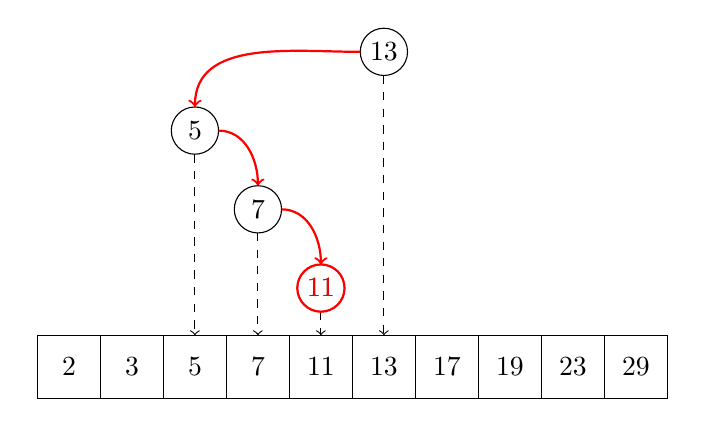
\begin{tikzpicture}
% draw the content of the array
\matrix (A) [matrix of nodes, nodes={draw, minimum size=8mm},
    column sep=-\pgflinewidth]{
    2 & 3 & 5 & 7 & 11 & 13 & 17 & 19 & 23 & 29\\};

% draw the elements, pointing at their source
\draw (-2,3)   circle (.3cm) node[align=center] {5};
\draw[->,thin,dashed] (-2,3-.3) -- (-2,0.4);

\draw (-1.2,2) circle (.3cm) node[align=center] {7};
\draw[->,thin,dashed] (-1.2,2-.3) -- (-1.2,0.4);

\draw (-.4,1)  circle (.3cm) node[align=center] {11};
\draw[->,thin,dashed] (-.4,1-.3) -- (-.4,0.4);

\draw (.4,4)   circle (.3cm) node[align=center] {13};
\draw[->,thin,dashed] (.4,4-.3) -- (.4,0.4);

% searching for 11
\draw [->,red,thick] (.4-.3,4)   to [out=180,in=90] (-2,3+.3);   % 13 to 5
\draw [->,red,thick] (-2+.3,3)   to [out=0,in=90]   (-1.2,2+.3); % 5 to 7
\draw [->,red,thick] (-1.2+.3,2) to [out=0,in=90]   (-.4,1+.3);  % 7 to 11
\draw [red,thick] (-.4,1)  circle (.3cm) node[align=center] {11};

\end{tikzpicture}


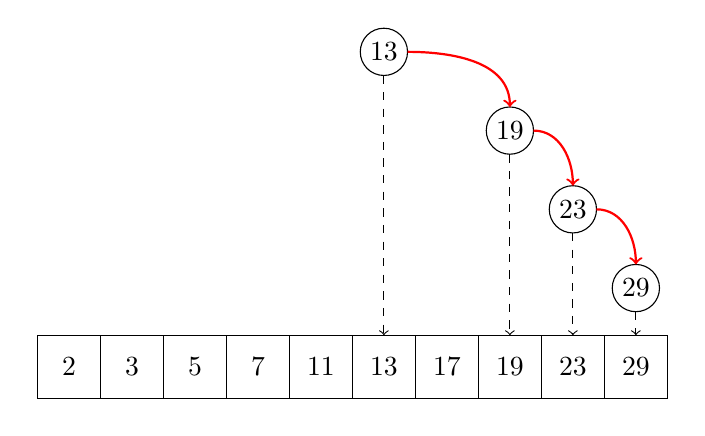
\begin{tikzpicture}
% draw the content of the array
\matrix (A) [matrix of nodes, nodes={draw, minimum size=8mm},
    column sep=-\pgflinewidth]{
    2 & 3 & 5 & 7 & 11 & 13 & 17 & 19 & 23 & 29\\};

% draw the elements, pointing at their source
\draw (.4,4)   circle (.3cm) node[align=center] {13};
\draw[->,thin,dashed] (.4,4-.3) -- (.4,0.4);

\draw (2,3)    circle (.3cm) node[align=center] {19};
\draw[->,thin,dashed] (2,3-.3) -- (2,0.4);

\draw (2.8,2)  circle (.3cm) node[align=center] {23};
\draw[->,thin,dashed] (2.8,2-.3) -- (2.8,0.4);

\draw (3.6,1)  circle (.3cm) node[align=center] {29};
\draw[->,thin,dashed] (3.6,1-.3) -- (3.6,0.4);

% searching for 31
\draw [->,red,thick] (2.8+.3,2)  to [out=0,in=90]   (3.6,1+.3);  % 23 to 29
\draw [->,red,thick] (2+.3,3)    to [out=0,in=90]   (2.8,2+.3);  % 19 to 23
\draw [->,red,thick] (.4+.3,4)   to [out=0,in=90]   (2,3+.3);    % 13 to 19

\end{tikzpicture}


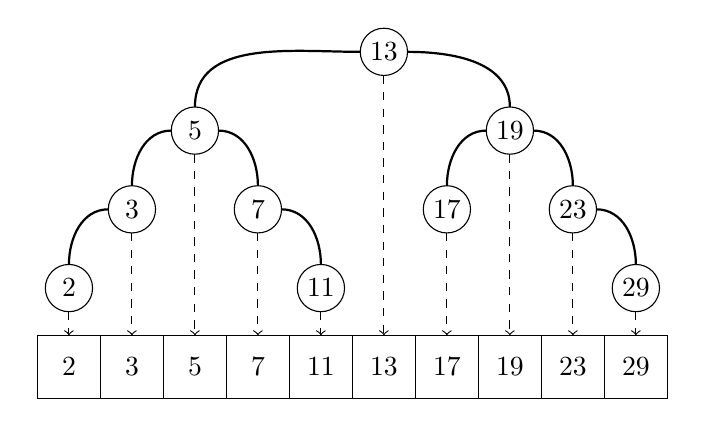
\begin{tikzpicture}
% draw the content of the array
\matrix (A) [matrix of nodes, nodes={draw, minimum size=8mm},
    column sep=-\pgflinewidth]{
    2 & 3 & 5 & 7 & 11 & 13 & 17 & 19 & 23 & 29\\};

% draw the elements, pointing at their source
\draw (-3.6,1) circle (.3cm) node [align=center] {2};
\draw[->,thin,dashed] (-3.6,1-.3) -- (-3.6,0.4);

\draw (-2.8,2) circle (.3cm) node[align=center] {3};
\draw[->,thin,dashed] (-2.8,2-.3) -- (-2.8,0.4);

\draw (-2,3)   circle (.3cm) node[align=center] {5};
\draw[->,thin,dashed] (-2,3-.3) -- (-2,0.4);

\draw (-1.2,2) circle (.3cm) node[align=center] {7};
\draw[->,thin,dashed] (-1.2,2-.3) -- (-1.2,0.4);

\draw (-.4,1)  circle (.3cm) node[align=center] {11};
\draw[->,thin,dashed] (-.4,1-.3) -- (-.4,0.4);

\draw (.4,4)   circle (.3cm) node[align=center] {13};
\draw[->,thin,dashed] (.4,4-.3) -- (.4,0.4);

\draw (1.2,2)  circle (.3cm) node[align=center] {17};
\draw[->,thin,dashed] (1.2,2-.3) -- (1.2,0.4);

\draw (2,3)    circle (.3cm) node[align=center] {19};
\draw[->,thin,dashed] (2,3-.3) -- (2,0.4);

\draw (2.8,2)  circle (.3cm) node[align=center] {23};
\draw[->,thin,dashed] (2.8,2-.3) -- (2.8,0.4);

\draw (3.6,1)  circle (.3cm) node[align=center] {29};
\draw[->,thin,dashed] (3.6,1-.3) -- (3.6,0.4);

% all of the possible arcs
\draw [thick] (2.8+.3,2)  to [out=0,in=90]   (3.6,1+.3);  % 23 to 29
\draw [thick] (2+.3,3)    to [out=0,in=90]   (2.8,2+.3);  % 19 to 23
\draw [thick] (2-.3,3)    to [out=180,in=90] (1.2,2+.3);  % 19 to 17
\draw [thick] (.4+.3,4)   to [out=0,in=90]   (2,3+.3);    % 13 to 19
\draw [thick] (.4-.3,4)   to [out=180,in=90] (-2,3+.3);   % 13 to 5
\draw [thick] (-1.2+.3,2) to [out=0,in=90]   (-.4,1+.3);  % 7 to 11
\draw [thick] (-2+.3,3)   to [out=0,in=90]   (-1.2,2+.3); % 5 to 7
\draw [thick] (-2-.3,3)   to [out=180,in=90] (-2.8,2+.3); % 5 to 3
\draw [thick] (-2.8-.3,2) to [out=180,in=90] (-3.6,1+.3); % 3 to 2

\end{tikzpicture}

\end{document}
